\section{Differentiation}

  Now, we will establish differentiation and culminate in the fundamental theorem of calculus. Monotone functions are a nice class of functions to study for differentiation and for constructing more general measures. 

  \begin{theorem}
    Suppose $f$ is monotone, increasing on $[a, b]$. Then, the set of discontinuities of $f$ at most countable. 
  \end{theorem}
  \begin{proof}
    Let $x_k$ be any point of discontinuity. Note that 
    \begin{equation}
      \lim_{x \to x_k^-} f(x), \qquad \lim_{x \to x_k^+} f(x)
    \end{equation}
    both exist by monotonicity, but since there is a discontinuity, we have 
    \begin{equation}
      L_k^- = \lim_{x \to x_k^-} f(x) < \lim_{x \to x_k^+} f(x) = L_k^+
    \end{equation}
    Then, $L_k^+ - L_k^-$ is a jump of $f$ at $x_k$. These intervals $[L_k^-, L_k^+]$ are disjoint due to monotonicity, and each interval contains a rational number. So there can only be at most countable intervals. 
  \end{proof}

  One piece of info from this trick. 

  \begin{definition}
    A point $x$ is a discontinuity of the first kind of $f(x)$ if both one-sided limits exist. 
  \end{definition}

  Now here's a generalization for not necessarily monotone functions. 

  \begin{theorem}[Detour]
    The set of discontinuities of the first kind is countable. 
  \end{theorem}
  \begin{proof}
    Idea of the proof. Look at some jump discontinuity and record the jump $\eta > 0$. Then, find $\delta > 0$ s.t. if $0 < y - x < \delta$, then 
    \begin{equation}
      \big| f(x)  - \lim_{y \to x^+} f(y) \big|  < \frac{\eta}{10}
    \end{equation}
    Then look at the rectangle on the graph associated with each jump. Because the limits exist, you can pick the rectangles so small that they are completely disjoint. Look at picture. 
  \end{proof}

  Now back to monotone functions. 

  \begin{theorem}
    For any countable set $C \subset (a, b)$ (where the interval doesn't need to be bounded), there exists monotonically increasing $f$ with a jump at each $x \in C$ and continuous at every $x \not\in C$. 
  \end{theorem}
  \begin{proof}
    Let $x_1, x_2, \ldots$ be $C$, and define 
    \begin{equation}
      f(x) = \sum_{x_k \leq x, x \in C} 2^{-k}
    \end{equation}
    The sum is increasing and convergent (since it's dominated by geometric series). $f$ also has a jump of $2^{-k}$ at every $x_k$. 

    Now we prove continuity. Suppose $x \not\in C$. Take $N \in \mathbb{N}$. Find $\delta_N > 0$ s.t. 
    \begin{equation}
      x_1, x_2, \ldots, x_N \not\in (x - \delta_N, x + \delta_N)
    \end{equation}
    which is possible since this is a finite set. The remaining sum can only add up to $2^{-N}$, and so $f(x + \delta_N) - f(x - \delta_N) \leq 2^{-N}$. 
  \end{proof}


\subsection{Oct 22} 

  \begin{theorem}[Fundamental Theorem of Calculus of Absolutely Continuous Functions]
    Suppose $f$ is AC on $[a, b]$.\footnote{Note that this is bounded and closed.} Then $f$ is differentiable a.e. on $(a, b)$, and $f^\prime$ is integrable on $[a, b]$, and 
    \begin{equation}
      \int_a^b f^\prime = f(b) - f(a)
    \end{equation}
  \end{theorem}

  An immediate corollary is that we can do 
  \begin{equation}
    \int_a^x = f(x) - f(a) \quad \forall x \in [a, b]
  \end{equation}
  If $f$ is AC on $[a, b]$, then $f$ is AC on $[a, x]$.  

  \begin{corollary}
    $f$ is AC on $[a, b]$ if and only if 
    \begin{equation}
      f(x) = f(a) + \int_a^x g(y) \,dy \quad \forall x \in [a, b]
    \end{equation}
    for some integrable $g$. 
  \end{corollary}
  \begin{proof}
    We prove bidirectionally. 
    \begin{enumerate}
      \item The forward implication is quite straightforward using the fundamental theorem. 
      \item $(\leftarrow)$ We just need to prove that the antiderivative is absolutely continuous. Take $\{(a_k, b_k)\}_{k=1}^n$ disjoint. We estimate the total variation,
        \begin{equation}
          \sum_{k=1}^n |f(b_k) - f(a_k)| 
        \end{equation}
        and try to make this small if the measure of the unions of the intervals is small. Just using the definition that $f$ is the antiderivative, the sum can be bounded by 
        \begin{equation}
          \sum_{k=1}^n |f(b_k) - f(a_k)| \leq \sum_{k=1}^n \int_{a_k}^{b_k} |g| \,dx = \int_{\cup (a_k, b_k)} |g| \,dx 
        \end{equation}
        using the triangle inequality, and then using additivity. The rest is just $\epsilon$-$\delta$ language. $\forall \epsilon > 0$, $\exists \delta > 0$ s.t. 
        \begin{equation}
          m(\bigcup (a_k, b_k)) < \delta \implies \sum_{k=1}^n |f(b_k) - f(a_k)| < \epsilon
        \end{equation}
        This is true since $g$ is integrable, and whenever the measure of the region that you are integrating on is less than $\delta$, your integral will be less than $\epsilon$. So $\exists \delta > 0$ s.t. for all measurable $E$, 
        \begin{equation}
          m(E) < \delta \implies \int_E |g| \,dx < \epsilon
        \end{equation}
        This is just the definition of integrability. This implies that 
        \begin{equation}
          \sum_{k=1}^n |a_k - b_k| < \delta \implies \sum_{k=1}^n |f(b_k) - f(a_k)| < \epsilon 
        \end{equation}
        Note that we are using the bounded 
    \end{enumerate}
  \end{proof}

  Another corollary is for monotone functions, and how we can determine whether they are AC or not. 

  \begin{corollary}[AC of Monotone Functions]
    Let $f$ be monotone on $[a, b]$. Then $f$ is AC if and only if 
    \begin{equation}
      \int_a^b f^\prime \,dx = f(b) - f(a)
    \end{equation}
    If we have montone function, note that derivative should exist a.e., and the derivative is integrable for monotone functions. Note that in the previous corollary, we need to check for all $x \in [a, b]$, but in here, we only need to check at the endpoints $a$ and $b$. 
  \end{corollary}
  \begin{proof}
    Bidirectional. 
    \begin{enumerate}
      \item $(\rightarrow)$. 
      \item $(\leftarrow)$. Let $x \in [a, b]$. We know from assumption---by rearranging the terms---that
      \begin{equation}
        0 = \int_a^b f^\prime - \big( f(b) - f(a) \big)
      \end{equation}
      But by additivity of the integral, we have 
      \begin{equation}
        = \underbrace{\int_a^x f^\prime - \big( f(x) - f(a) \big)}_{\leq 0} + \underbrace{\int_x^b f^\prime - \big( f(b) - f(x) \big)}_{\leq 0}
      \end{equation}
      But we know that WLOG, $f$ is increasing. If $f$ is increasing, then we know that both integrals should be positive, since the only type of discontinuities can be jump discontinuities. 
      \begin{equation}
        \int_a^x f^\prime - \big( f(x) - f(a) \big) + \int_x^b f^\prime - \big( f(b) - f(x) \big)
      \end{equation}

    \end{enumerate}
  \end{proof}

  This is another corollary, also sometimes known as the fundamental theorem for absolutely continuous functions. 

  \begin{lemma} 
    Le $f$ be integrable over $[a, b]$, with 
    \begin{equation}
      \int_{x_1}^{x_2} f\, dx = 0 \quad \forall (x_1, x_2) \subset [a, b]
    \end{equation}
    Then, $f = 0$ a.e. $[a, b]$. 
  \end{lemma}
  \begin{proof}
    Note that if we add the constraint that $f \geq 0$, then this is true. But the potential problem is that $f$ might change signs, which may cancel out. So starting from the assumption, we know that for any open $O$, 
    \begin{equation}
      \int_O f \,dx = 0 \quad \forall O \text{ open} 
    \end{equation}
    Since $G_\delta$ sets can be written as a decreasing sequence of open sets, by continuity of measure, we can write 
    \begin{equation}
      \int_G f \,dx = 0 \quad \forall G \text{ } G_\delta
    \end{equation}
    Since any measurable set $E$ can be written as $E = G \setminus E_0$ with $m(E_0) = 0$, we have 
    \begin{equation}
      \int_E f \,dx = 0 \quad \forall E \text{ measurable}
    \end{equation}
    So let $E^+ = \{ x \in [a, b] \mid f(x) > 0\}$ and $E^- = \{ x \in [a, b] \mid f(x) < 0\}$. So we have the first equalities
    \begin{align}
      0 & = \int_{E^+} f = \int_a^b f^+ \\
      0 & = \int_{E^-} f = - \int_a^b f^-  
    \end{align}
    So this means that $f^+ = f^- = 0$ a.e. 
  \end{proof}

  \begin{corollary}
    Let $f$ be integrable over bounded, closed interval $[a, b]$. Then, 
    \begin{equation}
      \frac{d}{dx} \bigg[ \int_a^x f \,dt \bigg] = f(x) \quad \text{ for a.e. } x \in (a, b)
    \end{equation}
    So basically, the derivative of the antiderivative is the function itself. 
  \end{corollary}
  \begin{proof}
    We know that $\int_a^x f \,dt$ is AC, so by two corollaries ago, its derivative must exist a.e. Let's call it $F(x) = \int_a^x f \, dt$, and so $F^\prime$ is integrable. So we need to compare $F^\prime$ and $f$. For any $(x_1, x_2) \subset [a, b]$ by linearity, we have 
    \begin{equation}
      \int_{x_1}^{x_2} [ F^\prime - f ] = \int_{x_1}^{x_2} F^\prime - \int_{x_1}^{x_2} f 
    \end{equation}
    where the integral of the first term is $F(x_2) - F(x_1)$, since it is AC. For the second term, we know that $F = \int_a^x f \,dt$, so can can split it 
    \begin{equation}
      = F(x_2) - F(x_1) - \underbrace{\int_a^{x_2}}_{F(x_2)} + \underbrace{\int_{a}^{x_1}}_{F(x_1)} = 0
    \end{equation}
    So this is true for any open interval in $[a, b]$. Then by invoking the previous lemma, $f = F^\prime$ a.e. 
  \end{proof}

  This is the end of absolutely continuous functions. 

\subsection{Oct 22. Convex Functions} 

  \begin{definition}[Convex Function]
    $\varphi$ is convex on $(a, b) \subset \mathbb{R}$ if $\forall x_1, x_2 \in (a, b)$, $\forall \lambda \in [0, 1]$, the linear interpolation 
    \begin{equation}
      \varphi (\lambda x_1 + (1 - \lambda) x_2) \leq \lambda \varphi(x_1) + (1 - \lambda) \varphi(x_2)
    \end{equation}
  \end{definition}

  Note that if we have $x = \lambda x_1 + (1 - \lambda) x_2$, then $\lambda = \frac{x_2 - x}{x_2 - x_1}$, and so the definition can be rewritten as 
  \begin{equation}
    \varphi(x) \leq \frac{x_2 - x}{x_2 - x_1} \varphi(x_1) + \frac{x - x_1}{x_2 - x_1} \varphi(x_2) \quad \forall x \in [x_1, x_2]
  \end{equation}
  Note that the two fraction coefficients add up to $1$. So we can write 
  \begin{equation}
    \frac{x_2 - x}{x_2 - x_1} \varphi(x) + \frac{x - x_1}{x_2 - x_1} \varphi(x)  \leq \frac{x_2 - x}{x_2 - x_1} \varphi(x_1) + \frac{x - x_1}{x_2 - x_1} \varphi(x_2) \quad \forall x \in (x_1, x_2)
  \end{equation}
  and rearranging, we get 
  \begin{equation}
    \frac{x_2 - x}{x_2 - x_1} \big( \varphi(x) - \varphi(x_1) \big) = \frac{x - x_1}{x_2 - x_1} \big( \varphi(x_2) - \varphi(x) \big)
  \end{equation} 
  Cancel out the common denominator to get 
  \begin{equation}
    \frac{\varphi(x) - \varphi(x_1)}{x - x_1} \leq \frac{\varphi(x_2) - \varphi(x)}{x_2 - x} \qquad \forall x \in (x_1, x_2)
  \end{equation}
  This is an if and only if derivation, so this is an equivalent. 

  \begin{theorem}
    If $\varphi$ is differentiable on $(a, b)$ with $\varphi^\prime$ increaseing, then $\varphi$ is convex. 
  \end{theorem}
  \begin{proof}
    Note that the LHS $= \varphi^\prime (c_1)$, RHS $= \varphi^\prime (c_2)$. Therefore, 
    \begin{equation}
      \varphi^\prime (c_1) \leq \varphi^\prime (c_2)
    \end{equation}
  \end{proof}

  \begin{example}
    $x^p$ for $p \geq 1$ is convex on $(0, \infty)$. Also, $e^{\alpha x}$ for $\alpha > 1$ is convex on $\mathbb{R}$. 
  \end{example}

  \begin{lemma}[Chorded Slope Lemma]
    Let $\varphi$ be convex on $(a, b)$, with $x_1 < x < x_2$ belonging to $a, b$. Then, 
    \begin{equation}
      \frac{\varphi(x) - \varphi(x_1)}{x - x_1} \leq \frac{\varphi(x_2) - \varphi(x_1)}{x_2 - x_1} \leq \frac{\varphi(x_2) - \varphi(x)}{x_2 - x} 
    \end{equation}
  \end{lemma}
  \begin{proof}
    Note that we can just write the second term as an interpolation of the first and third terms. 
    \begin{equation}
      \frac{\varphi(x_2) - \varphi(x_1)}{x_2 - x_1} = \frac{\varphi(x) - \varphi(x_1)}{x - x_1} \frac{x - x_1}{x_2 - x_1} + \frac{\varphi(x_2) - \varphi(x)}{x_2 - x} \frac{x_2 - x}{x_2 - x_1}
    \end{equation}
  \end{proof}

  \begin{theorem}
    Let $\varphi$ be convex on $(a, b)$. Then $\varphi$ has left and right derivatives at each point $x \in (a, b)$. Moreover, if $u < v$ on $(a, b)$, then 
    \begin{equation}
      \varphi^\prime (u^-) \leq \varphi^\prime (u^+) \leq \frac{\varphi(v) - \varphi(u)}{v - u} \leq \varphi^\prime (v^-) \leq \varphi^\prime (v^+)
    \end{equation}
  \end{theorem}
  \begin{proof}
    From lemma, $\varphi(u^-)$ exists since $\frac{\varphi(u) - \varphi(w)}{u - w}$ is monotonically incraesing in $w$. It is also bounded from above by $\frac{\varphi(v) - \varphi(u)}{v - u}$. So $\varphi^\prime(u^-)$ exists. 
  \end{proof}

\subsection{Oct 27: Convex Continued} 

  \begin{corollary}
    If $\varphi$ is convex on $[a, b]$, then $\varphi$ is Lipschitz, i.e.
    \begin{equation}
      | \varphi(x) - \varphi(y)| \leq M (x - y)  \quad \forall x, y \in [a, b], M = \max\{ |\varphi^\prime (a^+)|, | \varphi^\prime (b^-)| \}
    \end{equation}
    which hence implies that $\varphi$ is AC, and hence differentiable a.e.
  \end{corollary}

  This is quite nice, because we don't make any assumption on regularity for convex functions. But this tells us that not only is it continuous, but also Lipschitz. Since every Lipschitz function is also absolutely continuous, then convex functions are also absolutely continuous, and hence differentiable a.e.

  \begin{theorem}
    Suppose $\varphi$ is convex on $[a, b]$. Then, $\varphi$ is differentiable except on at most a countable set, and $\varphi^\prime$ is increasing. 
  \end{theorem}
  \begin{proof}
    Consider $\varphi(x^-)$, $\varphi (x^+)$. They are increasing in $x$ by the previous theorem. For monotone functions, we know that they can be discontinuous only on at most countable set.  So, these functions $\varphi^\prime (x^-), \varphi^\prime (x^+)$ are continuous except on perhaps at a countable set.\footnote{Considering jumps.} Let us denote it as $C$. Let us consider $x_0 \in [a, b] \setminus C$, and take a sequence $x_n \to x_0$, with $x_n \geq x_0$. Then, 
    \begin{equation}
      \varphi^\prime (x_0^-) \leq \varphi^\prime (x_0^+) \leq \frac{\varphi(x_n) - \varphi(x_0)}{x_n - x_0} \leq \varphi^\prime (x_n^-) 
    \end{equation}
    where $\varphi^\prime (x_n^-) \to \varphi^\prime (x_0^-)$ as $n \to +\infty$, since $x_0 \in [a, b] \setminus C$. So, $\varphi^\prime (x_0^-) = \varphi^\prime (x_0^+) \implies \varphi$ is differentiable at $x_0$. 
  \end{proof}

  \begin{definition}[Supporting Line]
    Let $\varphi$ be a convex. A \textbf{supporting line} at $(x_0, \varphi(x_0))$ is a lower function 
    \begin{equation}
      \ell (x) = a(x - x_0) + \varphi(x_0)
    \end{equation}
    satisfying $\varphi(x) \geq \ell(x)$ for all $x$. 

    \begin{figure}[H]
      \centering
      \begin{subfigure}[b]{0.48\textwidth}
        \centering
        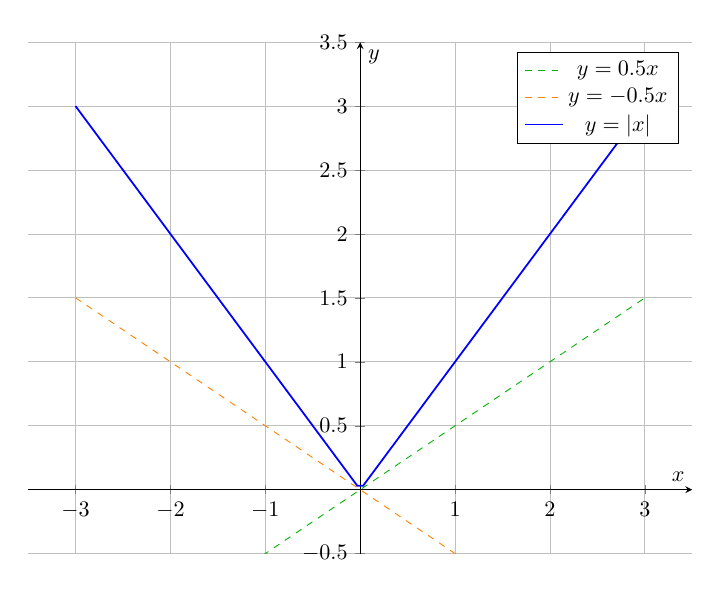
\begin{tikzpicture}[scale=0.8]
          \begin{axis}[
            axis lines=middle,
            xlabel={$x$},
            ylabel={$y$},
            domain=-3:3,
            samples=100,
            ymin=-0.5,
            ymax=3.5,
            xmin=-3.5,
            xmax=3.5,
            width=\textwidth,
            height=0.8\textwidth,
            grid=major,
            ]
            % Lines through origin (strictly below)
            \addplot[green!70!black, dashed, domain=-3:3] {0.5*x};
            \addplot[orange, dashed, domain=-3:3] {-0.5*x};
            % Absolute value function
            \addplot[blue, thick] {abs(x)};
            \legend{$y = 0.5x$, $y = -0.5x$, $y = |x|$}
          \end{axis}
        \end{tikzpicture}
        \caption{Absolute value function with linear bounds}
        \label{fig:absolute}
      \end{subfigure}
      \hfill 
      \begin{subfigure}[b]{0.48\textwidth}
        \centering
        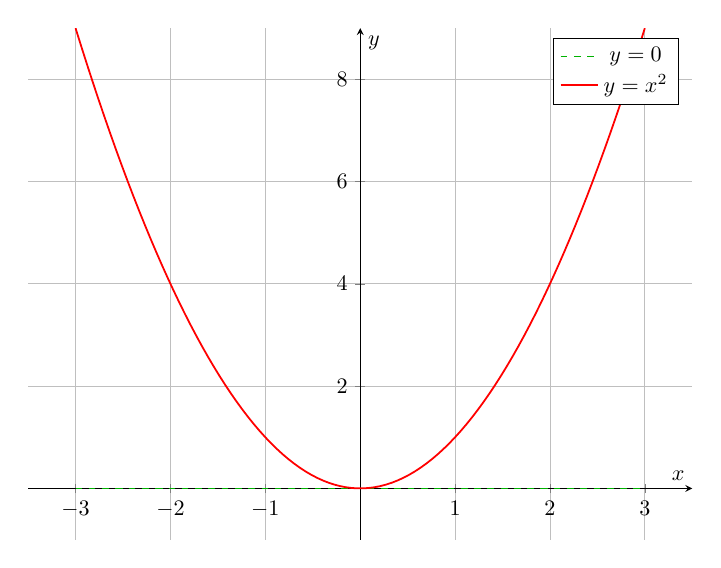
\begin{tikzpicture}[scale=0.8]
          \begin{axis}[
            axis lines=middle,
            xlabel={$x$},
            ylabel={$y$},
            domain=-3:3,
            samples=100,
            ymin=-1,
            ymax=9,
            xmin=-3.5,
            xmax=3.5,
            width=\textwidth,
            height=0.8\textwidth,
            grid=major,
            ]
            % Horizontal line through origin (strictly below)
            \addplot[green!70!black, dashed, domain=-3:3] {0};
            % Quadratic function
            \addplot[red, thick] {x^2};
            \legend{$y = 0$, $y = x^2$}
          \end{axis}
        \end{tikzpicture}
        \caption{Quadratic function with horizontal bound}
        \label{fig:quadratic}
      \end{subfigure}
      \caption{Basic mathematical functions with linear bounds through the origin}
      \label{fig:functions}
    \end{figure}
  \end{definition}

  Note that there can be multiple supporting lines. 

  \begin{theorem}[Jensen's Inequality]
    suppose $\varphi$ is convex on $\mathbb{R}$, with $f, \varphi \circ f$ integrable. Then, 
    \begin{equation}
      \varphi \bigg( \int_0^1 f \,dx \bigg) \leq \int_0^1 \varphi (f(x)) \,dx
    \end{equation}
  \end{theorem}
  \begin{proof}
    This first proof is good intuitively, but not a neat proof.  This is like the definition of convexity, but in a ``continuous  appearance.'' Note that we can think of these as Riemann sums, 
    \begin{equation}
      \varphi \bigg( \sum f_i \Delta x_i \bigg) \leq \sum_{i} \varphi_i \varphi(f_i) \Delta x_i
    \end{equation}
    and then you can pass through the limit to get the integral version. But this is a good intuition. 
  \end{proof}
  \begin{proof}
    The second proof is neater. Set $\alpha = \int_0^1 f\,dx$. Choose $k$ between $\varphi^\prime (\alpha^-), \varphi^\prime (\alpha^+)$. Then, the line 
    \begin{equation}
      \ell(x) \coloneqq k (x - \alpha) + \varphi(\alpha) 
    \end{equation}
    is supporting for $\varphi$, so $\varphi(x) \geq \ell(x)$. Also, $\varphi(f(x)) \geq \ell (f(x))$. Integrate 
    \begin{equation}
      \int_0^1 \varphi (f(x)) \,dx \geq \int_0^1 \Big( \underbrace{k (f(x) - \alpha)}_{= 0} + \varphi(\alpha) \Big) \,dx = \varphi \bigg( \int_0^1 f\,dx \bigg)
    \end{equation}
  \end{proof} 

  On $[a, b]$, we have to normalize $f$, 
  \begin{equation}
    \varphi \bigg( \frac{1}{b - a} \int_a^b f(x) \bigg) \leq \frac{1}{b - a} \int_a^b \varphi (f(x)) \,dx
  \end{equation}

\subsection{Lp Spaces}

  Suppose $E$ is measurable, and $f$ is measurable on $E$. Then, define 
  \begin{equation}
    \|f\|_p \coloneqq \bigg( \int_E |f|^p \bigg)^{1/p}, \qquad 1 \leq p < +\infty
  \end{equation} 
  This tells us more about the properties of the function, and how it may blow up or how its singularities might behave. 

  For $p = \infty$, we can define it as the maximum of the function (since by EVT). In general, we can define 
  \begin{equation}
    \|f\|_{\infty} \coloneqq \mathrm{esssup} |f(x)| \coloneqq \inf \{ M \mid |f(x)| \leq M \text{ a.e. } x\}
  \end{equation}

  The functions in $L^p$ don't really satisfy the norm property that $\|f\| = 0 \iff f =0$, so we can just consider equivalence classes of functions. For the subadditivity of the norm, checking for $p=1$ is the easiest, and also to some extend $p=\infty$. 

  \begin{definition}[Lp Space]
    Given $1 \leq p \leq +\infty$, define $L^p (E)$ to be the vector space of all $f$ measurable on $E$ s.t. $\int_E |f|^p < +\infty$. 
  \end{definition}
  \begin{proof}
    We first prove that it is a linear space. Since 
    \begin{equation}
      | f + g |^p \leq 2^p (|f|^p + |g|^p)
    \end{equation}
    so $f + g \in L^p$ if $f, g \in L^p$. 
  \end{proof}

  \begin{theorem}[Young's Inequality]
    Suppose $1 \leq p < +\infty$, with $q = \frac{p}{p-1}$, i.e. $\frac{1}{p} + \frac{1}{q} = 1$. Let $a, b \geq 0$. Then 
    \begin{equation}
      a b \leq \frac{a^p}{p} + \frac{b^q}{q} 
    \end{equation}
  \end{theorem}
  \begin{proof}
    Let the exponential function be $y = x^{p-1}$. Then, we get $x = y^{\frac{1}{p-1}}$. The proof is similar to if the function intersects the upper side of the rectangle. 

    \begin{figure}[H]
      \centering
      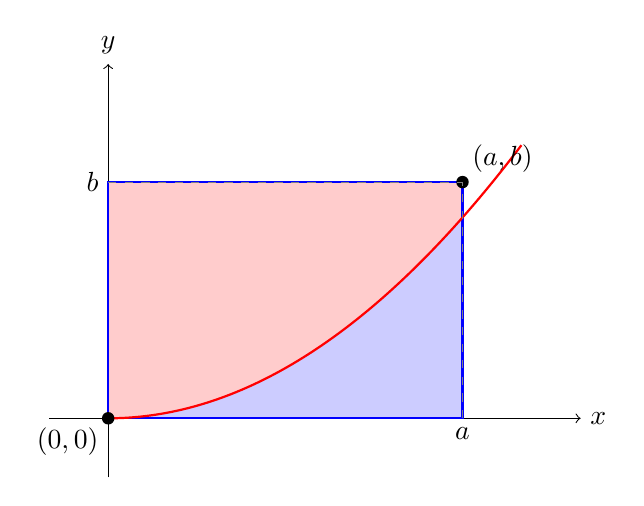
\begin{tikzpicture}[scale=1.5]
        % Draw axes
        \draw[->] (-0.5,0) -- (4,0) node[right] {$x$};
        \draw[->] (0,-0.5) -- (0,3) node[above] {$y$};
        
        % Define a and b
        \def\a{3}
        \def\b{2}
        
        % Shade area below the curve
        \fill[blue!20] (0,0) -- plot[domain=0:\a, samples=100] (\x, {1.7*(\x/\a)^2}) -- (\a,0) -- cycle;
        
        % Shade area above the curve
        \fill[red!20] plot[domain=0:\a, samples=100] (\x, {1.7*(\x/\a)^2}) -- (\a,\b) -- (0,\b) -- (0,0);
        
        % Draw rectangle
        \draw[blue, thick] (0,0) rectangle (\a,\b);
        
        % Draw exponential function extended beyond (a,b)
        \draw[red, thick, domain=0:3.5, samples=100] plot (\x, {1.7*(\x/\a)^2});
        
        % Label vertices
        \node[below left] at (0,0) {$(0,0)$};
        \node[above right] at (\a,\b) {$(a,b)$};
        
        % Mark points
        \fill (0,0) circle (1.5pt);
        \fill (\a,\b) circle (1.5pt);
        
        % Draw dashed lines to axes
        \draw[dashed, gray] (\a,0) -- (\a,\b);
        \draw[dashed, gray] (0,\b) -- (\a,\b);
        
        % Label axes values
        \node[below] at (\a,0) {$a$};
        \node[left] at (0,\b) {$b$};
      \end{tikzpicture}
      \caption{Rectangle with exponentially increasing curve and shaded regions}
      \label{fig:rectangle}
    \end{figure}

    We can see that the blue region has area 
    \begin{equation}
      \int_0^a x^{p-1} \,dx = \frac{a^p}{p} 
    \end{equation}
    We see that the red region has area $A$, 
    \begin{equation}
      A \leq \int_0^b y^{\frac{1}{p-1}} \,dy = \frac{y^{\frac{1}{p-1} + 1}}{\frac{1}{p-1} + 1} \bigg|_0^b = \frac{b^q}{q} 
    \end{equation}
  \end{proof}

  \begin{theorem}[Holder]
    Let $E$ be measurable, $1 \leq p \leq \infty$, $q = \frac{p}{p-1}$. Suppose $f \in L^p, g \in L^q$. Then, $f, g \in L^1 (E)$, and 
    \begin{equation}
      \int_E |fg| \,dx \leq \|f\|_p \|g\|_q
    \end{equation}
    In fact, this is sharp. If $f \neq 0$, then (note that this is the dual vector of $f$)
    \begin{equation}
      f^\ast (x) \coloneqq \|f\|_p^{1 - p} \mathrm{sgn}(f(x)) |f(x)|^{p-1} \in L^q
    \end{equation}
    with 
    \begin{equation}
      \|f^\ast \|_q = 1, \quad \int f f^\ast \,dx = \|f\|_p
    \end{equation}
  \end{theorem}
  \begin{proof}
    If $p =1$ ,or $p = \infty$, then this can be proven by monotonicity. If $1 < p < \infty$, then assume that $\|f\|_p = \|g\|_q = 1$, since by linearity, we can just normalize them by multiplying them by a constant. Not it suffices to prove that the integral $\leq 1$. Then, by Young's inequality,
    \begin{equation}
      |f(x) g(x)| \leq \frac{|f(x)|^p}{p} + \frac{|g(x)|^q}{q}
    \end{equation}
    and by integrating over $E$, since the RHS is integrable (it is also bounded?), we get 
    \begin{equation}
      \int_E |f(x) g(x)| \,dx \leq \frac{1}{p} + \frac{1}{q} = 1
    \end{equation}

    Finally, 
    \begin{equation}
      \|f^\ast\|_q^q = \|f\|_p^{(1-p) q} \int |f(x)|^{(p-1)q} \,dx = \|f\|_p^{-p} \int |f(x)|^p \,dx = 1
    \end{equation}
  \end{proof}

  \begin{corollary}[Cauchy-Schwartz]
    If $p = q = 2$, then we get Cauchy Schwartz. 
  \end{corollary}

  \begin{theorem}[Minkowski]
    If $f, g \in L^p$, then $f + g \in L^p$, and we get 
    \begin{equation}
      \| f + g \|_p \leq \|f\|_p + \|g\|_q
    \end{equation}
    This is the third condition for a norm. For $p = 1, +\infty$, this is immediate. Given $h \in L^p$, define 
    \begin{equation}
      h^\ast \coloneqq \|f\|_p^{1-p} \mathrm{sgn}(h) \, |h|^{p-1} 
    \end{equation}
    Then, from the previous theorem, 
    \begin{align}
      \| f + g \|_p & = \int_E (f + g)(f + g)^\ast \,dx  \\ 
                    & = \int_E f (f + g)^\ast \,dx + \int_E g (f + g)^\ast \,dx  \\ 
                    & \leq \|f\|_p \underbrace{\|(f + g)^\ast\|_q}_{1} + \|g\|_p \underbrace{\|(f + g)^\ast\|_q}_{1} 
    \end{align}
  \end{theorem}

  The following is an easy way to check that $\mathscr{F}$ is equi-integrable. 

  \begin{corollary}
    let $\mathscr{F}$ be a family of functions s.t. 
    \begin{equation}
      \int |f|^p \,dx < +\infty \forall f \in \mathscr{F}
    \end{equation}
    Then $\mathscr{F}$ is equi-integrable. 
  \end{corollary}
  \begin{proof}
    Let $A$ be ameasurable, $m(A) \leq \delta$. Then 
    \begin{equation}
      \int_A |f| \,dx \leq \bigg( \int_A |f|^p \bigg)^{1/p} \bigg( \int_A 1^q \bigg)^{1/q} \leq M^{1/p} m(A) \leq m^{1/p} \delta^{1/q} 
    \end{equation}
    Given any $\epsilon > 0$, we can choose $\delta > 0$ s.t. $\int |f| \,dx \leq \epsilon$ if $m(A) < \delta$. 
  \end{proof}

  \begin{corollary}
    Assume $E$ has finite measure. Then, $L^{p_1} \subset L^{p_2}$ for any $1 \leq p_1 \leq p_2 \leq +\infty$. So a higher exponent is more restrictive in a finite measure set. 
  \end{corollary}
  \begin{proof}
    A simple application of Holder's inequality. 
    \begin{equation}
      \int_E |f|^{p_1} \leq \bigg( \int_E |f|^{p_2} \,dx \bigg)^{p_1/p_2} x 
    \end{equation}
  \end{proof}

  In infinite measures, there are two ways that this can fail: singularities or tails. Either because it blows up, or it doesn't decay fast enough to be in $L^p$. $x^{-\alpha}$. 


\subsection{Nov 3} 

  \begin{example}
    Consider $f_m (x)$ in $L^p [0, 1]$, with 
    \begin{equation}
      f_m (x) =  \chi_{I_k^{(n)}} (x) \cdot 2^{n/p}, \quad I_k^{(n)} = [ (k-1) 2^{-n}, k 2^{-n}] 
    \end{equation}
    Note that $\|f_m\|_{L^p} = 1$, but $\|f_{m_1} - f_{m_2}\|_{L^p} \geq \frac{1}{2}$. So there are no limit points in $f_m$. 
  \end{example}

  \begin{definition}[Dual Vector]
    Suppose $X$ is a Banach space. Then $\mathcal{L}: X \to \mathbb{R}$ is called a \textbf{linear bounded functional} on $X$ if 
    \begin{equation}
      \mathcal{L}(\alpha f + \beta g)  = \alpha \mathcal{L} f + \beta \mathcal{L} g, \quad \forall f, g \in X
    \end{equation}
    and  
    \begin{equation}
      | \mathcal{L} (f)| \leq \|\mathcal{L}\|_\ast \|f\|, \quad \forall f \in X
    \end{equation}
  \end{definition}

  Whenever you want to prove that an integral is bounded, then you use Holder. 

  \begin{example}
    Let $X = L^p (E)$. Then 
    \begin{equation}
      \mathcal{L} f \coloneqq \int f g \,dx, \quad g \in L^q, q = \frac{p}{p - 1}
    \end{equation}
    is a linear bounded functional (by Holder). 
  \end{example}

  $L^\infty$ is not separable (as in there is no dense countable subset). 

  \begin{theorem}
    Given a Banach space $X$, the space of all linear bounded functionals on $X$ is a linear space with norm 
    \begin{equation}
      \|\mathcal{L}\|_\ast = \sup_{f \in X, \|f\| \leq 1} | \mathcal{L} (f) |
    \end{equation}
    This space is called \textbf{dual} to $X$, denoted $X^\ast$. 
  \end{theorem}
  \begin{proof}
    Just check that the sum, scalar multiplication is still a linear functional. Then for norm, just use triangle inequality. 
  \end{proof}

  We would like to prove that $(L^p)^\ast = L^q$, which we will do later. Now we'll define a different form of convergence. The regular pointwise convergence is known as strong convergence. 

  \begin{definition}[Weak Convergence]
    We say $f_n \rightharpoonup f$, i.e. \textbf{converges weakly} on $X$ if 
    \begin{equation}
      \mathcal{L}(f_n) \to \mathcal{L}(f), \quad \forall \mathcal{L} \in X^\ast
    \end{equation}
  \end{definition}


  \begin{example}
    Let $f_m(x)$ as before, and fix $g \in L^q [0, 1]$. Then, by Holder, 
    \begin{equation}
      \bigg| \int_0^1 \chi_{I_k^{(n)}} (x) g(x)\,dx  \bigg| \leq \|f_m\|_{L^p} \cdot \| g \cdot \chi_{I_k^{(n)}}\|_{L^q} \to 0, \text{ as } m \to +\infty
    \end{equation}
    since 
    \begin{equation}
      \int_{I_k^{(n)}} |g|^p \,dx \to 0 \text{ as } n \to +\infty
    \end{equation}
    by DCT, since $I_k^{(n)} = [(k-1) 2^{-n}, k 2^{-n}]$. 
  \end{example}

  So if we know that $(L^p)^\ast = L^q$, we could conclude $f_m \rightharpoonup 0$. 

  \begin{lemma}
    Suppose $\mathcal{L}_1, \mathcal{L}_2 \in X^\ast$. Suppose $Y$ is a dense subset of $X$. If $\mathcal{L}_1 = \mathcal{L}_2$ on $Y$, then $\mathcal{L}_1 = \mathcal{L}_2$. 
  \end{lemma}
  \begin{proof}
    Take any $g \in X$. Find $f \in Y$ s.t. $\|f - g\|_X \leq \epsilon$. Then, 
    \begin{align}
      |\mathcal{L}_1 g - \mathcal{L}_2 g| 
        & \leq |\mathcal{L}_1 g - \mathcal{L}_1 f| + \underbrace{|\mathcal{L}_1 f - \mathcal{L}_2 f|}_{=0} + |\mathcal{L}_2 f - \mathcal{L}_2 g| \\ 
        & \leq (\|\mathcal{L}_1\|_\ast + \| \mathcal{L}_2\|_\ast) \epsilon
    \end{align}
  \end{proof}

  \begin{lemma} 
    Let $E \subset \mathbb{R}$ be measurable, $1 \leq p \leq +\infty$. Suppose $g \in L^1 (E)$ and 
    \begin{equation}
      \bigg| \int_E f g \,dx \bigg| \leq M \| f\|_p, \quad \forall f \in L^p \text{ simple}
    \end{equation}
    Then, $g \in L^q, \|g\|_q \leq M$. 
  \end{lemma}
  \begin{proof}
    Consider $+\infty > p > 1$. Consider a sequence of simple $\varphi_n$ s.t. $\varphi_n \to |g|$ a.e., with $0 \leq \varphi_n \leq |g|$. Then, it suffices to show that 
    \begin{equation}
      \int | \varphi_n|^q \,dx \leq M, \quad \forall n
    \end{equation}
    since we can just invoke Fatou's lemma. Define simple $f_n = \mathrm{sgn}(g) |\varphi_n|^{q-1}$. Note $f_n \in L^p$ (simple functions). Then 
    \begin{equation}
      \int_E |\varphi_n|^q\,dx \leq  \int_E g \cdot f_n \,dx \leq M \|f_n \|_p, 
    \end{equation}
    where 
    \begin{equation}
      \|f_n\|_p = \bigg( \int | \varphi_n|^{q-1)p} \,dx \bigg)^{1/p} = \| \varphi_n \|_q^{q/p} 
    \end{equation}
    So $\| \varphi_n \|_q^{q- \frac{q}{p}} = \|\varphi_n\|_q \leq M$. Since $q(1 - \frac{1}{p}) = q \frac{1}{q} = 1$. 
  \end{proof}

  \begin{theorem}
    Let $[a, b]$ be a finite interval, with $1 \leq p < +\infty$. Suppose $\mathcal{L}$ is a linear bounded functional on $L^p([a, b])$. Then $\exists g \in L^q ([a, b])$ s.t. $\mathcal{L}f = \int_a^b f g \,dx$. 
  \end{theorem}
  \begin{proof}
    Suppose $p > 1$. Define $\phi(x) = \mathcal{L}(\chi_{[0, x]})$. We claim that $\phi$ is AC. Take $[a_k, b_k]_{k=1}^n$ disjoint in $[a, b]$. We have 
    \begin{equation}
      \sum_{k=1}^n |\phi(b_k) - \phi(a_k)|
    \end{equation}
    Given $\epsilon > 0$, we want to show that $\exists \delta >0$ s.t. 
    \begin{equation}
      \sum_{k=1}^n |b_k - a_k| \leq \delta \implies \sum_{k=1}^n |\phi(b_k) - \phi(a_k)| < \epsilon 
    \end{equation}
    But 
    \begin{align}
      \sum_{k=1}^n |\phi(b_k) - \phi(a_k)| & = \mathcal{L} \underbrace{\bigg( \sum_{k=1}^n \mathrm{sgn} \big( \phi(b_k) - \phi(a_k) \big) \chi_{[a_k, b_k]} \bigg)}_{f} \\ 
      & \leq \|\mathcal{L}\|_\ast \|f\|_p \\ 
      & = \|\mathcal{L}\|_\ast \bigg( \sum_{k=1}^n (b_k - a_k) \bigg)^{1/p}
    \end{align}
    Take $\delta = \big( \frac{\epsilon}{\|\mathcal{L}\|_\ast} \big)^{p}$
  \end{proof}

  So now that we have proved that $\phi$ is AC, we are almost in a position to use the lemma we proved before. Then, $\exists g \in L^1$ s.t. $\phi(x) = \int_a^x g(t) \,dt$ by fundamental theorem of calculus. Given ay $\chi_{[c, d]}$, we have 
  \begin{equation}
    \mathcal{L}(\chi_{c, d}) = \phi(d) - \phi(c) = \int_c^d g(t) \,dtjjA
  \end{equation}
  So $\mathcal{L} f$ and $\int g f \,dx$ coincide on step functions, and step functions are a dense set in $L^p$. We have 
  \begin{equation}
    \bigg| \int g f \,dx \bigg| \leq \|\mathcal{L}\|_\ast \|f\|_p 
  \end{equation}
  By the lemma, $g \in L^q$, with $\|g\|_q \leq \|\mathcal{L}\|_\ast$. 

  Note that this is \textit{not true} on $L^\infty$. Indeed $(L^1)^\ast = L^\infty$ (this is easier to prove), but $(L^\infty)^\ast \neq L^1$. But it is hard to construct a counterexample, and people use the Banach extension theorem to define such counterexamples. 

  \begin{theorem}[Riesz Representation Theorem]
    Let $E \subset \mathbb{R}$ be measurable, $1 \leq p < +\infty$. Suppose $\mathcal{L}$ is a bounded linear functional on $L^p$. Then $\exists g \in L^q$ s.t. 
    \begin{equation}
      \mathcal{L}(f) = \int_E g f \,dx, \quad \|g\|_q = \|\mathcal{L}\|_\ast
    \end{equation}
  \end{theorem}

  The dual of continuous functions is Steljes measures. 

  Now let's talk about weak convergence. This gives you some sort of compactness of a unit ball in $X^\ast$ with respect to the norm, which is basically sort of like weak convergence. 

  \begin{theorem}[Helley]
    Lt $X$ be a Banach space, separable. Suppose $\mathcal{L}_n \in X^\ast$ satisfy $\|L_n\|_\ast \leq M$ for all $n$. Then, $\exists n_k$ s.t. 
    \begin{equation}
      L_{n_k} (f) \to L (f), \quad \forall f \in X
    \end{equation}
  \end{theorem}
  \begin{proof}
    Let $(f_n)_{n=1}^\infty$ be a countable dense subset in $X$. Then, $\{\mathcal{L}_n f_1\}_{n=1}^\infty$ is ? $\implies \exists$ subsequence $s_{1, m}$ s.t. $\mathcal{L}_{s_{1, m}} f_1 \to a_1$. Also, we can choose a $s_{2, m}$ subsequence of $s_{1, m}$ s.t. $\mathcal{L}_{s_2, m} f_2 \to a_2$, and so in $s_{l, m}$ s.t. 
    \begin{equation}
      \mathcal{L}_{s_{l, m}} f_j \to a_j, \quad \forall 1 \leq j \leq l
    \end{equation}
    Select $n_k = S_{k, k}$. Then, $\mathcal{L}_{n_k} f_j \to a_j$ for all $j$. Given any $g \in X$, consider 
    \begin{equation}
      |\mathcal{L}_{n_{k_2}} g - \mathcal{L}_{n_{k_1}} g| \leq |\mathcal{L}_{n_{k_2}} g - \mathcal{L}_{n_{k_1}} f| + |\mathcal{L}_{n_{k_2}} f - \mathcal{L}_{n_{k_1}} f| + |\mathcal{L}_{n_{k_2}} f - \mathcal{L}_{n_{k_1}} g|
    \end{equation}
    Fix $\epsilon > 0$, choose $f$ s.t. 
    \begin{equation}
      \|f - g\| \leq \frac{\epsilon}{3 \max\{\|f\|, \|g\|\}}
    \end{equation}
    Then, $k_1, k_2$, large so middle term $\leq \frac{\epsilon}{3}$. 
  \end{proof}

  So this is what people mean by a unit ball in $L^p$ is weakly compact. 

